
\chapter{Particle Finite Element Methods for the shallow water equations}
\label{lagrangian_sw}




In the previous chapter the SW equations have been analyzed considering the coupled convective and oscillatory mechanisms in an Eulerian framework. However, in some regions of the domain, the solution of the equations can be convection dominated. Specifically, where there is a movement of the shoreline --like run-up or flooding--, the problem is convection dominated.
This mechanism suggests the use of Lagrangian strategies, which have been successfully applied to convection diffusion and Navier-Stokes problems.

In this chapter, the developments of the Particle Finite Element Method (PFEM) are applied to the SW equations. The basis of the PFEM family of methods consists on a splitting operator, solving two stage fashion the convective operator and the rest of the equations. In the case of the SW equations, there is a stage for convection and other stage for wave mechanism.
The main advantage of the PFEM lies in using the variational principle of FEM. Hence, the formulations presented in chapter \refeq{eulerian_sw} are applicable with small modifications. The novelty of the PFEM consists on solving the convection with a particle method.

In the family of PFEM there are two main groups, the moving mesh and the fixed mesh. The mesh moving algorithm was firstly presented to the scientific community \cite{idelsohn2003,PFEM2004} and has been widely applied to a high number of situations \cite{larese2008,Salazar2012,onate2008}. In this method, the particles traditionally coincides with the nodes. After the convection stage --and eventually, remeshing--, the mesh inherits the displacements of the convection. Those displacements are part of the material derivative involved in the variational principle of the equations.

Lately, a second generation of the PFEM was presented \cite{idelsohn2012}. It uses a fixed mesh and is known as PFEM-2. The main idea consists on decoupling the particles from the nodes, leading to a duality of spaces: the FEM discretization and the particles discretization. Its main drawback is the introduction of projections between the two spaces but the cost of the projection is expected to be recovered by the use of a fixed mesh strategy without remeshing \cite{idelsohn2015,puigferrat2021}.



\section{Introduction}

The Lagrangian formulation starts by the definition of the material derivative. Let $\varphi$ be a scalar or vector property, the material derivative is obtained by applying the chain rule:
\begin{subequations} \label{mat_derivative}
\begin{align}
\frac{D}{Dt}\varphi(\mathbf{x},t) &= \pder{\varphi}{t} + u\cdot\nabla\varphi \label{mat_derivative:deriv} \\
\pder{\mathbf{x}}{t} &= \mathbf{u} \label{mat_derivative:conv}
\end{align}
\end{subequations}
The Lagrangian procedure consist on solving separately the equations (\ref{mat_derivative:deriv}) and (\ref{mat_derivative:conv}). To apply this staggered procedure, a generic conservation balance is considered,
\begin{equation} \label{conserv_balance}
\pder{\varphi}{t} + \nabla \mathbf{F} = 0
\end{equation}
where $\mathbf{F}$ is the fluxes vector in an infinitesimal volume of control. The balance equation is split into the convective and non convective fluxes, $\mathcal{L}_1$ and $\mathcal{L}_2$ respectively.
\begin{equation} \label{spatial_balance_linearized}
    \pder{\varphi}{t} + \mathcal{L}_1 \varphi + \mathcal{L}_2 \varphi = 0
\end{equation}
After introducing equation (\ref{mat_derivative}) into (\ref{spatial_balance_linearized}), the following expression is obtained,
\begin{equation} \label{mat_balance_liearized}
    \frac{D\varphi}{Dt} + \mathcal{L}_2 \varphi = 0
\end{equation}

Finally, the numerical strategy for solving a balance equation (\ref{conserv_balance}) in a Lagrangian framework consists on applying a splitting, generally, the first order Godunov splitting \cite{leveque2002} or the second order Strang splitting \cite{macnamara2016}.
The order of accuracy of the splitting operator is related to the sequence and the mode how equations (\ref{mat_derivative:conv}) and (\ref{mat_balance_liearized}) are temporally integrated.





\section{Mesh moving methods}


The PFEM method has been widely applied to solve the incompressible Navier-Stokes equations, especially with free surface problems \cite{larese2008}, multi-fluids \cite{mier2010} and fluid-structure interaction \cite{onate2008}.
The moving mesh allows to fit the sub-domains with the discretization and the boundaries are tracked in a natural way.
When the PFEM is applied to the SW equations, the mesh moving will be solving the water domain in the horizontal plane. That is, the moving shoreline in the SW equations is playing the role of the free surface in the NS equations.

Once the discretization describes and follows the fluid motion --$\eta$ and $\mathbf{u}$--, there appears the need to introduce another discretization to define the fixed topography and its variations --$z$--, since it does not move with the fluid. The duality of discretizations introduce the need of a mapping between the two meshes. The topography data need to be mapped to the computational mesh for solving the equations. And the primal variables need to be mapped to the topographical mesh for visualization purpose. See figure \ref{pfem_dual_mesh}, where the fluid domain $\Omega_w$ si inside the computational domain $\Omega$. The topographic domain $\Omega_T$ coincides with the computational domain $\Omega$.
This approach presents some analogies with embedded formulations, except on the fact that the discontinuity is on the fluid --computational domain-- instead of the topography --geometric domain--.


\begin{figure} [ht]
    \centering
    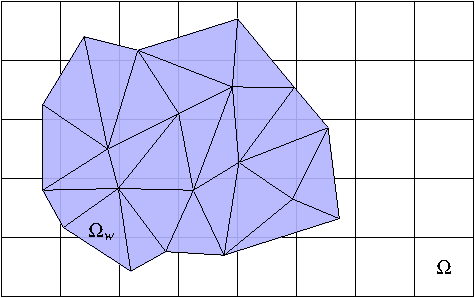
\includegraphics[width=.6\textwidth]{img/lagrangian/dual_pfem_mesh.pdf}
    \caption{Spatial discretization for the mesh moving PFEM algorithm.}
    \label{pfem_dual_mesh}
\end{figure}

Going back to the definition of the SW flow, the set of particles moving in the Lagrangian frame, convect the intrinsic properties (density, water depth, velocity, flow rate, etc.). The equations follow an \emph{updated lagrangian} formulation, that is, the variables are assumed to be known at time $t$ but unknown for the time $t+\Delta t$. Given that the variational principle is used to solve the equations in the continuum media, those is identified with the fluid domain, excluding the dry part. Once the convection is solved and the shoreline is updated, the system of equations is solved again.

Some modifications to this procedure may be considered. For example, an excessive deformation of the elements, without inverting them, may require a remeshing step. In that case, the identification of the shoreline coincides with the previous time step, but the interior domain will be refined. With a proper mesh quality control, the remeshing step can be applied only to those steps which really need it.

Additionally, an iterative scheme can be introduced, since the solution of the nwe system of equations at time step $t + \Delta t$ modifies the integration of the convective term. Usually this outer iteration loop is skipped by an explicit approximation of the convective term. The full path of the solution procedure is resumed in figure \ref{sw_pfem_algorithm}.

\begin{figure} [ht]
    \centering
    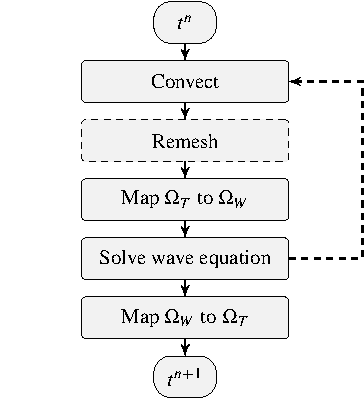
\includegraphics[width=.6\textwidth]{img/lagrangian/sw_pfem_algorithm.pdf}
    \caption{PFEM algorithm for the SW equations.}
    \label{sw_pfem_algorithm}
\end{figure}





\subsection{Governing equations}


Given that the nodes of the SW discretization are particles, the intrinsic properties are in a Lagrangian frame, thus, both mass and momentum balances follow a Lagrangian formulation. This fact reduces the non-linearity of the system of equations to be solved, making them easier to solve. On the other hand, in the Lagrangian framework the convection can be evaluated in terms of the primitive variables. We will take advantage of this characteristic to solve the primitive SW, which are more linear than the conservative ones.
The accuracy of the solutions obtained with the proposed method will be compared against the methods presented in the previous chapter.

Let the conservative vector of unknowns $\bm\phi$ be expressed in terms of the primitive set of variables $\bm\psi$. we recover the SW equations in terms of the primitive variables:
\begin{subequations}
\begin{align}
    \pder{\mathbf{u}}{t} &= \mathbf{u} \cdot \nabla \mathbf{u} + g \nabla(h-z_b) + g\mathbf{S}_f = \mathbf{0} \\
    \pder{h}{t} &= \mathbf{u} \cdot \nabla h + h \nabla \mathbf{u} = 0
\end{align}
\end{subequations}
The introduction of the material derivative definition yields
\begin{subequations} \label{pfem_mat_balance}
\begin{align}
    \frac{D\mathbf{u}}{Dt} &= g \nabla(h-z_b) + g\mathbf{S}_f = \mathbf{0} \\
    \frac{Dh}{Dt} &= h \nabla \mathbf{u} = 0
\end{align}
\end{subequations}

Analogously to the previous sections, if the solution $\psi$ is sufficiently smooth, it will also verify the quasilinear form
\begin{equation} \label{pfem_mat_balance_lin}
    \frac{D\bm{\psi}}{Dt} + \mathbf{A}_i\pder{\bm{\psi}}{x_i} + \mathbf{S}\bm{\psi} + \mathbf{T} = 0
\end{equation}
Where the matrix $\mathbf{S}$ and the vector $\mathbf{T}$ are the same than those defined in section \ref{equations}. The tangent matrices $\mathbf{A}_i$ have a new expression for this case, according to the change of variables and to the material derivative. The null diagonal corresponds to the non-convective look of the equations.
\begin{equation}
    \mathbf{A}_1 = \left[\begin{array}{ccc}
        0 & 0 & g \\
        0 & 0 & 0 \\
        h & 0 & 0
    \end{array}\right] \quad , \quad
    \mathbf{A}_2 = \left[\begin{array}{ccc}
        0 & 0 & 0 \\
        0 & 0 & g \\
        0 & h & 0
    \end{array}\right]
\end{equation}


The eigenvalues of $\mathbf{A}_i$ for the one-dimensional case are $\lambda = \pm c$, being $c=\sqrt{gh}$ the surface waves speed. These eigenvalues differ from $u+c$ and $u-c$ since we are in a Lagrangian frame, moving at velocity $u$.
For the two-dimensional case, the eigenvalues for each direction are obtained projecting $\mathbf{A}_i$ onto a unit vector and are always $-c$, $0$ and $c$.
The system is still hyperbolic and the positivity of $h$ is required. 




\subsection{Variational principle}


Despite the non-convective look of (\ref{pfem_mat_balance}), they need stabilization because of the incompatibility of the interpolation \cite{codina2008}. The fic-based stabilization method from \cite{onate1998} and from the previous sections will be reused. As stated before, this formulation presents a significative simplification with respect to the conservative equations in an Eulerian frame. The residual of the equations is defined as
\begin{equation}
    \mathbf{r} \defeq \frac{D\bm{\psi}}{Dt} + \mathbf{A}_i\pder{\bm{\psi}}{x_i} + \mathbf{S}\bm{\psi} + \mathbf{T} = 0 \quad i = 1,2
\end{equation}

The number of dimensions is $n_d=2$ and the number of balance equations is $n_b=3$. The FIC-balance using a first order expansion of Taylor series has the following expression:
\begin{equation} \label{fic_expression}
    r_j - \frac{1}{2} l^e \frac{\mathbf{A}_i}{\lambda_{max}} \pder{r_j}{x_i} = 0 \qquad i \in \{1,n_d\} \ , \ j \in \{1,n_b\}
\end{equation}
To introduce stability in the desired direction, the characteristic element length $l^e$ has been projected onto the normalized characteristics of the equation, $\mathbf{A}_i/\lambda_{max}$.
In practice, the term $\frac{1}{2}$ is replaced by an algorithmic constant $\beta$ in order to control the amount of extra diffusion. This parameter will be analyzed latter.


The resulting SW FIC-based stabilization is obtained from (\ref{pfem_mat_balance_lin}) and (\ref{fic_expression}). The variational principle is obtained by multiplying the FIC balance by a test function $\omega_k$ and integrating over the domain $\Omega_w$.
\begin{equation} \label{variational_fic_lagr}
    \int_{\Omega_w} \left(\omega_k \mathbf{r} + \omega_k \beta l^e \frac{\mathbf{A}_i}{\lambda} \pder{\mathbf{r}}{x_i}\right) d\Omega = 0
\end{equation}


\textcolor{red}{The second term of Equation (\ref{variational_fic_lagr}) is integrated by parts.} Note that the geometries are linear and the element length $l^e$ and the linearization matrix $\mathbf{A}_i$ are defined constant inside the element. Hence, the boundary integral which appears after integration by parts should be understood as the boundary of all the elements

\begin{equation} \label{variational_fic_lagr_parts}
\int_{\Omega_w} \omega_k \mathbf{r} d\Omega
- \int_{\Omega_w} \beta l^e\frac{\mathbf{A}_i}{\lambda}\pder{\omega_k}{x_i} \mathbf{r} d\Omega
+ \sum_e \int_{\Gamma_e} \beta l^e\frac{\mathbf{A}_i}{\lambda}\omega_kn_k \mathbf{r} d\Gamma = 0
\end{equation}
In this work we neglect the boundary integrals assuming that the residual $\mathbf{r}$ is null at the boundary of the elements. At this point we introduce the balance Equation (\ref{pfem_mat_balance}) and integrate by parts again. The result is

\begin{multline} \label{variational_balance_fic_lagr}
\int_{\Omega_w} \left(
    \omega_k \pder{\bm{\psi}}{t} + \omega_k \mathbf{A}_i\pder{\bm{\psi}}{x_i}
    + \pder{\omega_k}{x_j} \mathbf{K}_{jk} \pder{\bm{\psi}}{x_i} + \mathbf{S}\bm{\psi} + \mathbf{F}
\right) d\Omega\\ -
\int_{\Omega_w} \frac{\beta l^e}{\lambda} \left(
    \pder{\omega_k}{x_j} \mathbf{A}_j \pder{\bm{\psi}}{t}
    + \pder{\omega_k}{x_j} \mathbf{A}_j\mathbf{A}_i\pder{\bm{\psi}}{x_i}
    + \ppder{\omega_k}{x_j} \mathbf{A}_j\mathbf{K}_{jk} \pder{\bm{\psi}}{x_i} \right. \\
    \left.
    + \pder{\omega_k}{x_j} \mathbf{A}_j(\mathbf{S}\bm{\psi} + \mathbf{F})
\right) d\Omega
=0
\end{multline}
Equation (\ref{variational_balance_fic_lagr}) is the stabilized variational form for the shallow water equations, similar to the expression obtained by SUPG. Note that the parameter $\beta l^e/\lambda$ is analogous to the characteristic time $\tau$ of the classical SUPG or GLS techniques \cite{cotela2016}.



\subsection{Convective operator}


Apart from solving Eq. (\ref{pfem_mat_balance}), Eq. (\ref{mat_derivative:deriv}) needs to be integrated in time. Given that (\ref{mat_derivative:deriv}) does not involve a spatial derivatives, there is no need to use a variational principle and can be evaluated nodally. In other words, the trajectory of the particles is decoupled from the wave.

In order to evaluate the trajectory of the particles, Eq. (\ref{mat_derivative:deriv}) is rewritten in integral form
\begin{subequations}
\begin{align}
    \mathbf{x}(t^{n+1}) &= \mathbf{x}(t^n) + \int_{t^n}^{t^{n+1}} \mathbf{u}(t) dt \\
    \mathbf{u}(t^{n+1}) &= \mathbf{u}(t^n) + \int_{t^n}^{t^{n+1}} \mathbf{a}(t) dt
\end{align}
\end{subequations}


As far as the time variable is evaluated at discrete intervals $t = t^1, \dots t^n$, the continuous value of $t$ is not known. Therefore, a generic finite difference can be used to evaluate the position continuously in time:
\begin{equation}
    \mathbf{x}^{n+1} = \mathbf{x}^n +
        (1-\theta) (\Delta t \mathbf{u}^n + \frac{1}{2} \Delta t^2 \mathbf{a}^n) +
        \theta (\Delta t \mathbf{u}^{n+1} + \frac{1}{2} \Delta t^2 \mathbf{a}^{n+1})
\end{equation}
The fact of using the velocity interpolated is related to the coupled nature of equations (\ref{mat_derivative:deriv}) y (\ref{pfem_mat_balance}). The choose of an implicit or explicit finite differencing depends on the splitting and the iterative scheme.




\subsection{Limitations of the method}

The main advantage of this method consists on the possibility of solving convective problems with the primitive equations, specially when there is a moving shoreline. However, the major limitation is faced on the inner discontinuities, since the semi-implicit convection operator may invert elements. This problem is not solved with remeshing because the nodal values will resort on a wrong interpolation of the variables. Figure \ref{pfem_shock} shows a graphical representation of the strong conditions $CFL<1$ in order to prevent the inversion of elements.

\begin{figure} [htb]
    \centering
    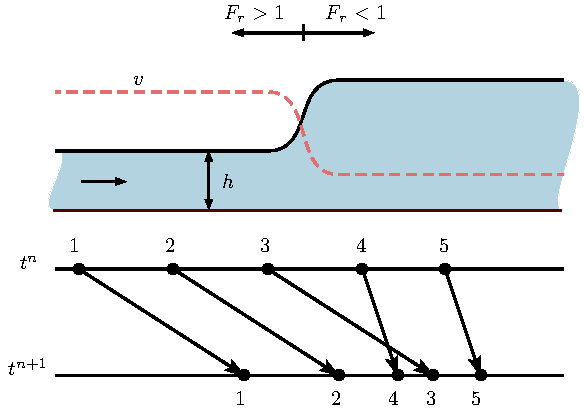
\includegraphics[width=.8\textwidth]{img/lagrangian/pfem_shock.pdf}
    \caption{Incompatibility of the mesh moving algorithm for solving problems with shocks.}
    \label{pfem_shock}
\end{figure}

While the primitive variables are not optimal to solve shocks, the mesh moving algorithm presents another difficulty.
Both methods present restrictions, but the nature of that difficulties are different. The restriction of the primitive variables is related to the conservation of the momentum at discrete level. The restriction of the mesh moving algorithm is associated to the finite differencing convective operator.



\subsection{Examples}


\section{Fixed mesh methods}

A diferencia del algoritmo tradicional PFEM, las partículas no coinciden con los nodos, sino que se mueven libremente sobre la malla de elementos finitos. Tiene la ventaja de no necesitar un remallado, pero el coste de definir una proyección para trasladar la información la malla de elementos finitos a las partículas.

En primer lugar, se define un conjunto de partículas que ocupan el dominio de aguas poco profundas. La densidad de partículas será tal que, habrá más partículas que elementos para el mismo dominio. Estas partícluas se desplazan transportando las propiedades intrínsecas (densidad, calado, velocidad, caudal, etc.). Después de la fase de desplazamiento, se proyectan las variables intrínsecas a la malla de elementos finitos, dando paso a la solución de un sistema de ecuaciones en un marco Lagrangiano. Es importante recalcar que para ello no se ha requierido ningún movimiento de la malla, pero sí la definición de una proyección. Esta primera proyección es trivial, ya que se emplea la interpolación de los elementos finitos.


%La información de la malla de elementos finitos se puede proyectar fácilmente a las partículas utilizando las funciones de forma. Sin embargo, la proyección de las partículas a la malla de elementos finitos requiere la definición de otra proyección.

%Estas partículas que se ha introducido, después de desplazarse, proyectan las variables intrínsecas a la malla de elementos finitos, dando paso a la solución de un sistema de ecuaciones en un marco Lagrangiano. Es importante recalcar que para ello no se ha requierido ningún movimiento de la malla, pero sí la definición de una proyección.

Un vez resuelto el sistema de ecuaciones, las partículas actualizan las variables características. Esta segunda proyección es un paso crítico, pues resulta necesario definir una proyección de los elementos a als partículas. Esta explicación resume brevemente el esquema de funcionamiento de una iteración no lineal. Usualmente, suele emplearse una sola iteración.

Igual que en el algoritmo de malla móvil, este esquema puede sufrir algunas variaciones, pues, en sentido estricto, se trata de un esquema implícito que requiere iterar entre en paso de convección y la resolución del sistema de ecuaciones. Dejamos el análisis del sistema de integración temporal para más adelante.


\subsection{Ecuaciones de gobierno}

A diferencia del algoritmo de malla móvil, los nodos reciben la información característica de la nueva configuración, sin que la malla se haya desplazado. Este hecho permite utilizar arbitrariamente un esquema Lagrangiano o Euleriano, independientemente de cómo se haya resuelto la convección. A la luz de esta consideración, es importante ver que la expresión de la conservación de la masa en un esquema Euelriano es trivial cuando se consideran variables conservativas. De este modo, consideramos la formulación Lagrangiana solamente en el balance de cantidad de movimiento. Otra posibilidad sería emplear las mismas ecuaciones de gobierno que en el caso de PFEM de malla móvil.

La aplicación de la regla de la cadena al operador convectivo nos lleva a la introducción de un nuevo término en el balande de cantidad de movimiento. Este término corresponde a la compresibilidad del flujo. Es importante recordad la analogía entre las ecuaciones de flujo compresible y las ecuaciones aguas poco profundas. Con tal de linealizar la solución del sistema de ecuaciones, se presentan tres vías que serán estudiadas:
\begin{itemize}
    \item Incluir el término de transporte compresible en el sistema de ecuaciones. Esta es la solución más consistente, sin embargo, la mas costosa ya que introduce una no linealidad y teŕminos que deben ser incluidos en la estabilización.
    \item Calcular el término compresible mediante la divergencia de los desplazamientos. Puesto que en la etapa de convección se calculan los desplazamientos, se dispone de los elementos necesarios para calcular la divergencia, modificando así la proyección de las variables intrínsecas a la malla de elementos finitos.
    \item Si la importancia relativa del presente término lo permite, omitirlo. Esta alternativa práctica, requiere la evaluación de aplicabilidad.
\end{itemize}


\subsection{Conclusiones}

Los métodos Lagrangianos presentan un esquema que permite un ahorro computacional. La gran ventaja que tienen es la facilidad para tratar el movimiento de la líne de costa o el avance de una inundación, evitando todos los problemas derivados de tener que incluir el dominio seco en el cálculo. El principal inconveniente de los métodos Lagrangianos está originado en que el campo de velocidades es discontínuo cuando hay un resalto hidráulico. Así como la discontinuidad que presenta la línea de costa queda resuelta de modo natural en los métodos Lagrangianos, la discontiuidad de los resaltos hidráulicos puede llevar a la inversión de elementos o proyecciones inadecuadas. Este aspecto necesita de técnicas específicas en los que la solución puede ser muy sensible al método utilizado, o puede ser poco robusta.

Por lo general, ante la presencia de resaltes hidráulicos, son preferibles los esquemas de integración temporal explícitos, frente a los implícitos. Puesto que la derivada no está definida en las discontinuidades, los esquemas semi-implícitos pueden llevar a soluciones que no convergen.




\section{Examples}



\section{Concluding remarks}


